\scanpage{5}
\mspage{4}

requires that if $U$ \deleted{$(=C\unsure{)(|(}T)$} is both finite tame
and cofinite tame, thus if $S$ and $T$
are \deleted{two} disjoint finite tame subsets
\deleted{such} such that \deleted{\unsure{every}} \inserted{a)} $S\cup T$
tame i.e. \figure{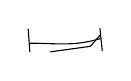
\begin{tikzpicture}[x=1cm,y=1cm]
\draw (0,.16)--(.02,-.13) (.91,.17)--(.94,-.12);
\draw (.01,-.02) to[out=0,in=197] (.92,.04);
\draw (.28,-.13)--(.79,-.06)--(.91,.08);
\end{tikzpicture}} $\unsure{s|S}\in S$ tame with respect to every
$t\in T$, and b) Every $u\in\mathcal L$ \unsure{tame|tame} with respect to
$S$ is in $T$\unsure{;|,}, \deleted{then $S\cup T=\mathcal L$} and
a fortiori $S\cup T$ is a maximal \inserted{finite} tame
subset, thus $S\cup T=\mathcal L$, and
$\unsure{{}^{\cdot\cdot}S_0|S_0}=P_2(\mathcal L)$, finally the equivalence
relations are discrete, and the
$\dot A$ are empty. To formulate it,
one defines \unsure{the|a}

\deleted{Definition} \inserted{Example 1} \uline{discrete \inserted{Network} structure} on $\mathcal L$

\[
 S_0=P_2(\mathcal L)\ \Longrightarrow\
 \left\{\begin{aligned}
 &\mathrm{Modf}(\unsure{\mathcal L|\mathcal L_0})=\deleted{\unsure{\mathrm{Mod}}}P_f(\mathcal L)\\
 &C_T=\mathcal L\setminus T\qquad\text{if }T\in P_f(\mathcal L)
 \end{aligned}\right.
\]

\[
\begin{aligned}
 &\deleted{C(T)=\unsure{\subset|\mathcal L}}\\
 &R_{\unsure{T|T\rceil|\Pi}}=\text{discrete equivalence relation}\\
 &\hspace{3em}\text{in }\mathcal L\setminus T,\quad\text{thus the components}\\
 &\hspace{4em} \inserted{A}\ \text{are reduced to a point}\\
 &\deleted{\text{For Thus}}\\
 &\dot A=\varnothing
\end{aligned}
\]

\uline{Axiom}\quad If $T$ is a maximal finite tame
subset, then $T=\mathcal L$, $\mathcal L$ is \unsure{discrete|discrete|discrete}.

% paper watermark, visible from the reverse
% the paper's watermark (EXTRA STRONG), not his text
